\documentclass[10pt]{article}

% ---- NeurIPS style ----
\usepackage{neurips_2026}

% ---- Packages ----
\usepackage[utf8]{inputenc}
\usepackage[T1]{fontenc}
\usepackage{amsmath,amssymb,amsfonts}
\usepackage{graphicx}
\usepackage{booktabs}
\usepackage{hyperref}
\usepackage{natbib}
\usepackage{xcolor}
\usepackage{multirow}
\usepackage{subcaption}
\usepackage{microtype}
\usepackage{enumitem}
\usepackage{wrapfig}

% Allow more floats per page
\renewcommand{\topfraction}{0.85}
\renewcommand{\textfraction}{0.1}
\setcounter{topnumber}{3}

\hypersetup{
  colorlinks=true,
  linkcolor=blue!70!black,
  citecolor=green!50!black,
  urlcolor=blue!70!black
}

% Compact lists
\setlist{nosep,leftmargin=*}

% Placeholder marker
\newcommand{\todo}[1]{\textcolor{red!70!black}{\textbf{[TODO: #1]}}}

\title{Where Teachers Teach:\\Position as the Signal Indicator in On-Policy Distillation}

\author{Anonymous Author(s)}

\begin{document}
\maketitle

% ===========================================================================
% ABSTRACT
% ===========================================================================
\begin{abstract}
On-policy distillation (OPD) trains a student to match a teacher on the student's own samples by minimizing reverse KL token-by-token. The default loss weights every generated token equally; we ask: \emph{among all generated tokens, which ones actually carry the distillation signal?} Holding the per-response budget fixed at $K{=}100$ tokens, we benchmark three families of selectors against the full-sequence loss on MATH-500: top-$K$ by per-token KL, three entropy-based variants (top-$K$ student entropy, top-$K$ teacher entropy, learned format-mask), and a contiguous prefix of the first $N$ positions. Top-KL underperforms full-seq by 3.75\,pp despite covering 93\% of the per-token KL mass between the \emph{initial} student and teacher; entropy variants all land within $\pm 1$\,pp of full-seq; only \emph{prefix-$K$ exceeds full-seq}, by 3.5--4.3\,pp on math. Position is not a coverage proxy: middle-100 and last-100 fall \emph{below} the no-distill baseline.

Prefix-$K$ improves over full-sequence in 7 of 9 cells we test across model families (Qwen, Gemma, Llama), training methods (LoRA, FullFT), and tasks (math, code, BFCL function calling); the two cells where prefix is not the winner are FullFT-math (loses by 1.5\,pp) and Llama BFCL (where neither full-seq nor prefix-$K$ beats the teacher). It cuts wall-clock by $\sim$10$\times$ and peak memory by $\sim$4$\times$, requires a one-line code change, and exhibits a single elbow at $N \approx 50$--150. On BFCL function calling, prefix-$K$ students exceed their teachers in two of three pairs (by 5.9--7.3\,pp). We give two interpretations consistent with the data: a cascade by which prefix supervision auto-aligns the tail (verified by tail-KL drop and a prefix-swap experiment), and mode-seeking reverse-KL on a contiguous prefix concentrating the student on a high-conviction trajectory mode.
\end{abstract}

% ===========================================================================
% 1. INTRODUCTION
% ===========================================================================
\section{Introduction}
\label{sec:intro}

On-policy distillation \citep{agarwal2024onpolicy,gu2024minillm,deepseekr1} trains a student on its own samples scored by a stronger teacher, and is now a workhorse for transferring reasoning and structured-output capabilities into smaller models. The standard objective is a \emph{token-wise} reverse KL averaged over all positions of each on-policy trajectory. The default weighting---one per token---bakes in the assumption that every position contributes equally to the supervision signal.

This assumption is empirically fragile. Across our experiments, full-sequence OPD often degrades during training: with three seeds for Qwen2.5-Math-1.5B$\to$Qwen3-1.7B on MATH-500, mean accuracy is $56.78 \pm 6.1$\,pp and one seed falls \emph{below} the no-distill baseline; for Gemma-2-2B$\to$Gemma-3-4B math, full-seq sits at 11.70\% against a 13.45\% no-distill baseline; for Llama-3.2-1B$\to$Llama-3.1-8B function calling, full-sequence distillation ends 23.3\,pp \emph{below} the raw student (raw 55.3\%, post-distill 32.0\%); for Qwen coding, HumanEval degrades from 39\% to 32\% over training. These are not implementation bugs---they are symptoms of a structural problem with the assumption that all token positions carry equal supervision value.

\textbf{The question.} Rather than patch the loss with a hand-crafted reweighting, we ask: \emph{which tokens carry the distillation signal?} We split the question into a head-to-head comparison among three plausible answers, holding the per-response budget fixed at $K{=}100$ tokens:

\begin{itemize}
\item \textbf{KL}: select the top-$K$ tokens with highest per-token KL---a natural divergence-based choice.
\item \textbf{Entropy}: top-$K$ by student or teacher entropy, or a learned \emph{format-mask} that drops low-entropy format tokens.
\item \textbf{Position}: the first $K$ tokens of each response (prefix-$K$).
\end{itemize}

A good indicator should at least \emph{exceed} full-sequence training; anything below full-seq is a strict regression---you would be better off using every token.

\textbf{Findings.} Only position passes that bar. On MATH-500 with the canonical Qwen pair (Table~\ref{tab:headline}), top-KL-100 underperforms full-seq by 3.75\,pp despite covering 93\% of total per-token KL mass; the three entropy variants land within $\pm 1$\,pp of full-seq; prefix-$K$ exceeds full-seq by 3.5--4.3\,pp at $N \in \{50, 100, 150, 200\}$. Negative controls (middle-100, last-100) fall \emph{below} no-distill, ruling out the hypothesis that the gain is just a coverage effect. The prefix wins despite covering only 46\% of per-token KL mass.

\textbf{Generality.} Prefix-$K$ matches or improves over full-sequence across model families (Qwen, Gemma, Llama---in two of three, full-sequence \emph{collapses}), tasks (math, code, BFCL), and methods (LoRA, full fine-tuning); the one cell where prefix loses is FullFT-math (Table~\ref{tab:generality}). It is also $\sim$10$\times$ faster wall-clock, $\sim$4$\times$ smaller in peak GPU memory, requires a one-line code change, and shows a single performance elbow at $N \approx 50$--150 across tasks. On BFCL function calling, students trained with prefix-$K$ \emph{exceed} their teachers in two of three pairs (by 5.9--7.3\,pp).

\textbf{Contributions.} (1)~The first head-to-head comparison of KL-, entropy-, and position-based selectors in OPD at fixed budget, revealing that only position exceeds full-sequence. (2)~Negative controls (middle/last) showing that late-token training is \emph{actively harmful}---worse than no distillation. (3)~Cross-family / cross-task / cross-method validation, including stability and efficiency. (4)~A cascade-plus-mode-seeking explanation backed by a tail-KL drop without tail training, a prefix-swap experiment, and token-level statistics from \texttt{signal\_analysis/range\_summary.json}.

% ===========================================================================
% 2. SETUP
% ===========================================================================
\section{Setup}
\label{sec:setup}

\textbf{On-policy distillation.} The student $p_\theta$ samples a response $y \sim p_\theta(\cdot \mid x)$; the teacher $q_\phi$ scores every position. The default loss is a sum of per-position reverse KL over the full response of length $T$:
\begin{equation}
\mathcal{L}_{\text{full}}
= \mathbb{E}_{y \sim p_\theta(\cdot|x)} \left[\sum_{t=1}^{T} D_{\mathrm{KL}}\!\left(p_\theta(\cdot \mid x, y_{<t}) \,\|\, q_\phi(\cdot \mid x, y_{<t})\right)\right].
\label{eq:fullseq}
\end{equation}
A token \emph{selector} replaces the uniform sum by a sum over a subset $\mathcal{S}(x,y) \subseteq \{1,\dots,T\}$ of size $K$: $\mathcal{L}_\mathcal{S} = \mathbb{E}\left[\sum_{t \in \mathcal{S}} D_{\mathrm{KL}}(\cdot)\right]$. We compare:
\begin{itemize}
\item \textbf{Top-KL-$K$}: $\mathcal{S}$ is the top-$K$ positions by $D_{\mathrm{KL}}(p_\theta\|q_\phi)$ on the sampled trajectory.
\item \textbf{Top-Ent-Student-$K$}, \textbf{Top-Ent-Teacher-$K$}: top-$K$ by student / teacher entropy.
\item \textbf{Format-mask}: drop low-entropy format tokens above a learned threshold (heuristic for ``style'' tokens).
\item \textbf{Random-$K$}: a $K$-uniform-random subset (control).
\item \textbf{Prefix-$K$}: $\mathcal{S} = \{1,\dots,K\}$, the first $K$ generated tokens.
\item \textbf{Middle-$K$}, \textbf{Last-$K$}: contiguous middle / final $K$ positions (negative controls).
\end{itemize}

\textbf{Notation.} $K$ denotes the per-response selector budget; for prefix-$K$, $K=N$ (the prefix length). Outside of selector tables we use $N$ to emphasize the contiguous-prefix view, and $K$ where contrast with non-prefix selectors is the point. ``Pos-200tok'' is a prefix selected by token-count rather than position-index; in our setting they coincide for tokenizer-aligned prompts and we use the labels interchangeably.

\textbf{Models.} The canonical pair is Qwen2.5-Math-1.5B \citep{qwen2024qwen25math} as student, Qwen3-1.7B \citep{qwen2025qwen3} as teacher; we also use Gemma-2-2B$\to$Gemma-3-4B and Llama-3.2-1B$\to$Llama-3.1-8B for cross-family results.

\textbf{Training.} LoRA \citep{hu2022lora} with $r=32$, $\alpha=64$ on $\{q,k,v,o,\text{gate},\text{up},\text{down}\}$\_proj; learning rate $5\times 10^{-5}$; 200 steps; 3200 problems; $n=1$ on-policy sample per problem; effective batch size 16 (\textbf{n1bs16}). Generation temperature 0.7. We also report full fine-tuning (FullFT) results. For position-restricted runs, we additionally clamp \texttt{max\_new\_tokens} to $N$, which is where most of the wall-clock savings come from.

\textbf{Evaluation.} MATH-500 \citep{lightman2023verify,hendrycks2021measuring} reported as avg@4 / maj@4 / pass@4 with $n=4$ samples at $T=0.7$; HumanEval / MBPP \citep{chen2021evaluating,austin2021program} via \texttt{evalplus}; BFCL function-calling full-accuracy. The undistilled student baselines are 50.95\% (Qwen math), 13.45\% (Gemma math), and 15.20\% (Llama math). The full-sequence number for the canonical Qwen pair is 62.35\%.


% ===========================================================================
% 3. PART 1: COMPARING SIGNAL INDICATORS
% ===========================================================================
\section{Part 1: What is a Good Signal Indicator?}
\label{sec:part1}

We hold $K=100$ fixed and ask which selector exceeds the full-sequence baseline. Table~\ref{tab:headline} is the headline result; Figure~\ref{fig:signal} visualizes it.

\begin{table}[t]
\centering
\caption{\textbf{Selector head-to-head, MATH-500 avg@4, n1bs16 LoRA, $K{=}100$.} Only the contiguous prefix \emph{exceeds} full-sequence. Negative controls (middle/last) fall below the no-distill baseline. KL coverage = fraction of total per-token reverse KL between the \emph{initial} student and teacher selected by the indicator on held-out trajectories; not invariant under training.}
\label{tab:headline}
\small
\begin{tabular}{@{}lrrr@{}}
\toprule
\textbf{Selector} & \textbf{avg@4} & \textbf{$\Delta$ vs full-seq} & \textbf{KL covered} \\
\midrule
No-distill baseline                & 50.95          & $-$11.40        & ---     \\
Middle-100 \textcolor{red!70!black}{(below baseline)} & 47.80 & $-$14.55 & $\sim$30\% \\
Last-100   \textcolor{red!70!black}{(below baseline)} & 50.35 & $-$12.00 & $\sim$15\% \\
\midrule
Top-KL-100                          & 58.60          & $-$3.75         & 93.2\%   \\
Top-Ent-Student-100                 & 61.35          & $-$1.00         & 67.0\%   \\
Format-mask                         & 62.05          & $-$0.30         & ---      \\
Top-Ent-Teacher-100                 & 62.20          & $-$0.15         & 50.5\%   \\
Full-sequence                       & 62.35          & 0.00            & 100.0\%  \\
Random-100                          & 63.05          & $+$0.70         & 21.1\%   \\
\midrule
Pos-100                             & 65.85          & $+$3.50         & 45.6\%   \\
Pos-200tok                          & 66.05          & $+$3.70         & ---      \\
\textbf{Pos-50} / \textbf{Pos-150}  & \textbf{66.65} & \textbf{$+$4.30}& ---      \\
\bottomrule
\end{tabular}
\end{table}

\begin{figure}[t]
  \centering
  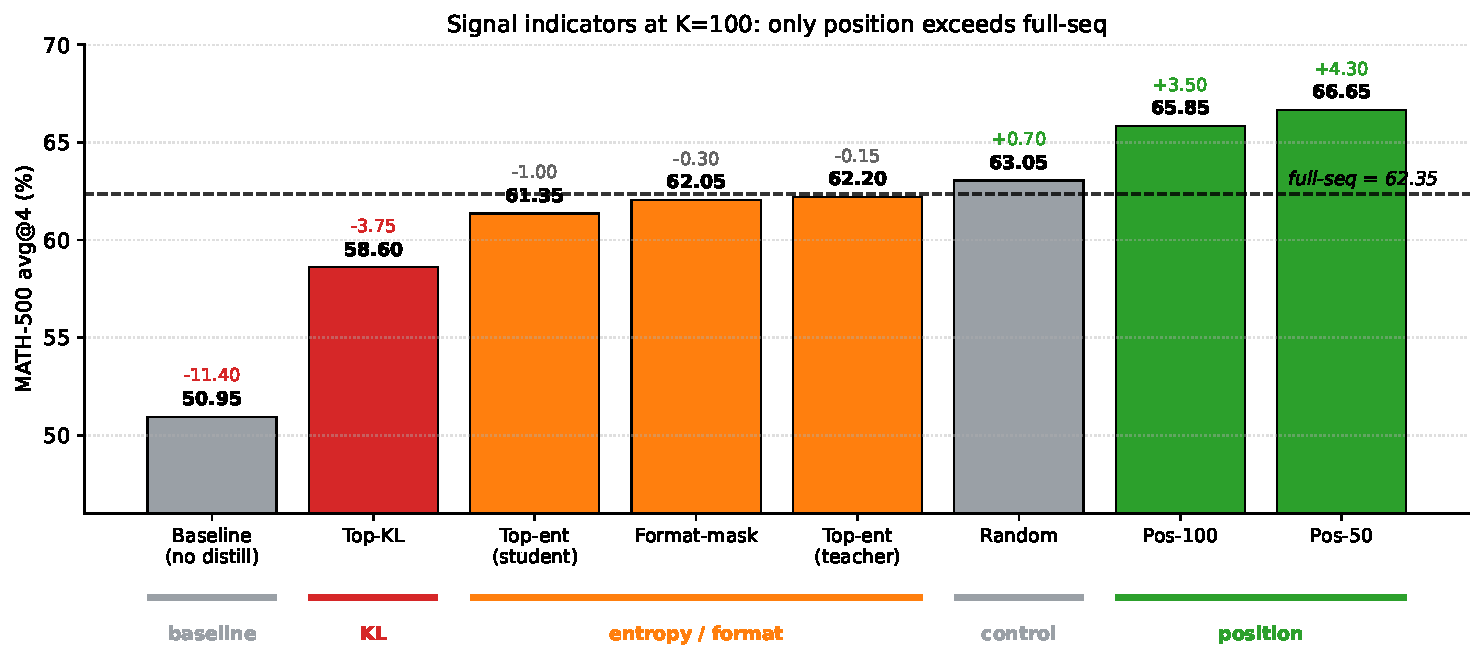
\includegraphics[width=0.85\textwidth]{figures/fig3_signal_indicators.pdf}
  \caption{\textbf{Signal indicators at fixed $K{=}100$.} Bars show MATH-500 avg@4 for each selector; the dashed line is full-sequence. Top-KL underperforms; entropy variants tie; only prefix exceeds. Negative controls fall below baseline.}
  \label{fig:signal}
\end{figure}

\subsection{KL is the Wrong Indicator}
\label{sec:kl_paradox}

The most natural indicator---rank tokens by their reverse KL---underperforms full-sequence by 3.75\,pp, despite covering more than 90\% of total per-token KL mass. Token classification (Table~\ref{tab:token_class_main}) explains why: the highest-KL tokens are dominated by LaTeX format and structural style, not reasoning. The category \texttt{math\_latex} (e.g., \texttt{\textbackslash(}, \texttt{\textbackslash[}, \texttt{\textbackslash\textbackslash}) has mean KL 3.99---more than 10$\times$ that of digits and operators. Training the student on these positions teaches it how the teacher \emph{types}, not how it \emph{thinks}.

\begin{table}[h]
\centering
\caption{\textbf{Token classification at high-KL positions.} Highest-KL = format / style disagreement, not reasoning quality.}
\label{tab:token_class_main}
\small
\begin{tabular}{@{}llr@{}}
\toprule
\textbf{Category} & \textbf{Example tokens} & \textbf{Mean KL} \\
\midrule
math\_latex (format)     & \texttt{\textbackslash(}, \texttt{\textbackslash[}, \texttt{\textbackslash\textbackslash} & 3.99 \\
planning                 & ``To'', ``First'', ``Therefore''                                                  & 1.75 \\
structural               & \texttt{**}, \texttt{:}, newlines                                                  & 0.89 \\
math\_operator           & $=, +, -$                                                                         & 0.38 \\
math\_number             & 0--9                                                                              & 0.28 \\
\bottomrule
\end{tabular}
\end{table}

\textbf{Takeaway.} High KL is a divergence metric; it is not, by itself, a teaching signal.

\subsection{Entropy: Necessary, Not Sufficient}
\label{sec:entropy}

If high-KL fails because LaTeX format dominates, then entropy---which downweights low-entropy format tokens---should win. It does not. The three entropy-based selectors (top-$K$ student entropy, top-$K$ teacher entropy, format-mask) all land within $\pm 1$\,pp of full-sequence (Table~\ref{tab:headline}). They strip out the worst format tokens that hurt top-KL but do not exceed full-seq. Even random-$K$ matches full-seq---suggesting full-sequence's number is a \emph{floor} for any non-pathological selector that avoids format-dominated tokens, not a ceiling.\footnote{We deploy entropy and confidence as fixed-budget hard selectors here; the cited works in \S\ref{sec:concurrent} use them as soft reweightings of the full-sequence loss. The two are not interchangeable, and our claim is the narrower one (\S\ref{sec:concurrent}, ``Scope of comparison'').}


\textbf{Why entropy ties.} Entropy ranks tokens by local uncertainty, which loosely correlates with where the teacher has something to teach. But a high-entropy token \emph{late} in a trajectory sits on a path that has already drifted; aligning it does not fix the answer. A high-entropy token \emph{early} sets the trajectory; aligning it can fix everything downstream. Top-entropy weights both equally, washing out to full-sequence behavior.

\subsection{Position Uniquely Exceeds Full-Sequence}
\label{sec:position_wins}

Prefix-$K$ is the simplest possible selector: take the first $K$ generated tokens. It exceeds full-sequence by 3.5--4.3\,pp at $K \in \{50,100,150,200\}$ and is the only selector with this property in our experiments.

\textbf{Position is not just a high-entropy region.} If position were \emph{only} entropy-correlated, hard top-entropy-$K$ should match prefix-$K$. The 4.5\,pp gap (61.35 vs.\ 65.85) shows it does not. Inside the head (Appendix~\ref{app:surprise}): the first 50 tokens are 2.4$\times$ enriched in the top global surprise quartile but still contain 13.1\% bottom-quartile tokens; even head-500 covers only 31.8\% of the top quartile. Position is correlated with entropy, not equivalent to it.

\textbf{Why does the contiguous prefix dominate?} We see two effects, taken up in detail in Section~\ref{sec:why}:

\begin{enumerate}
\item \textbf{Causal coverage.} Aligning the planning prefix re-orients the entire trajectory; aligning scattered late tokens does not (cascade evidence: \S\ref{sec:cascade}).
\item \textbf{Distribution-shape coupling.} A contiguous prefix matches the autoregressive structure of the model: every gradient step aligns the conditional $p_\theta(y_t \mid y_{<t})$ at the same context the model actually decodes from at inference. Mode-seeking reverse-KL on this prefix concentrates the student on a single high-conviction trajectory mode (\S\ref{sec:surpass}).
\end{enumerate}

\textbf{Bridge to Part 2.} The Part 1 result is established on a single setting (Qwen-math, n1bs16 LoRA, $K{=}100$). Before unpacking the mechanism, we test how broadly it survives: across model families, tasks, training methods, seeds, and choices of $N$.

% ===========================================================================
% 4. PART 2: POSITION IS A GREAT STRATEGY
% ===========================================================================
\section{Part 2: Robustness of the Part 1 Claim}
\label{sec:part2}

Part 1's head-to-head was on one pair, one task, and one seed configuration. This section tests whether the prefix-$K$ wins survive across model families, tasks, training methods, seeds, and choices of $N$, and whether they come with practical efficiency benefits worth caring about.

\subsection{Main Results}
\label{sec:main_results}

Table~\ref{tab:math_main} reports MATH-500 results for the canonical pair across selectors and position settings.

\begin{table}[t]
\centering
\caption{\textbf{MATH-500 (Qwen2.5-Math-1.5B$\to$Qwen3-1.7B, n1bs16 LoRA).} Prefix-$K$ improves over full-seq by 3.5--4.3\,pp on avg@4 and 4.3--7.4\,pp on pass@4. Best step among checkpoints \{50, 100, 150, 200\}.}
\label{tab:math_main}
\small
\begin{tabular}{@{}lrrrr@{}}
\toprule
\textbf{Method} & \textbf{Best step} & \textbf{avg@4} & \textbf{maj@4} & \textbf{pass@4} \\
\midrule
No-distill         & ---  & 50.95 & 61.20 & 72.80 \\
Top-KL-100         & 50   & 58.60 & 65.80 & 74.40 \\
Top-Ent-Student-100& 100  & 61.35 & 67.20 & 73.20 \\
Format-mask        & 50   & 62.05 & 67.20 & 76.20 \\
Top-Ent-Teacher-100& 150  & 62.20 & 67.80 & 75.80 \\
Full-sequence      & 150  & 62.35 & 69.40 & 74.60 \\
Random-100         & 150  & 63.05 & 69.20 & 76.80 \\
Pos-100            & 200  & 65.85 & 70.80 & 79.80 \\
Pos-200tok         & 50   & 66.05 & 71.20 & 81.00 \\
\textbf{Pos-50}    & 150  & \textbf{66.65} & 71.00 & \textbf{81.00} \\
\textbf{Pos-150}   & 100  & \textbf{66.65} & 67.00 & \textbf{81.00} \\
\bottomrule
\end{tabular}
\end{table}

\textbf{Coding (HumanEval, LoRA).} On the coding task, LoRA full-sequence \emph{degrades} from 40.2 (step 50) to 26.8 (step 400)---a 13.4\,pp drop over training. Prefix-$K$ is stable: pos-50 reaches 42.1 (HE) / 36.6 (HE+) at step 350; pos-100 reaches 42.1 / 36.0 at step 150. Full results in Appendix~\ref{app:coding}.

\textbf{Negative controls.} Middle-100 reaches only 47.80\,pp---3.15\,pp \emph{below} the no-distill baseline---and last-100 reaches 50.35, also below baseline (Table~\ref{tab:headline}). The contrast with prefix-100 (65.85) cannot be explained by training-budget or coverage arguments alone: the same number of tokens placed in different parts of the response yield differences of $>$15\,pp. Training on late tokens is not just less useful---it is \emph{actively harmful}.

\subsection{Generality: Cross-Family, Cross-Task, Cross-Method}
\label{sec:generality}

Table~\ref{tab:generality} sweeps families, tasks, and methods. Three observations: (i)~prefix-$K$ wins on math for every family, in two cases where full-sequence \emph{collapses below baseline}; (ii)~prefix-$K$ matches or wins on coding and BFCL function calling, with one BFCL pair (Llama, Table~\ref{tab:funcall}) where prefix falls 4.7\,pp below the teacher; (iii)~the one cell where prefix \emph{loses} is FullFT-math (56.75 vs.\ 58.20, $-$1.45\,pp). CoT (``thinking'') mode shows the same pattern as plain decoding: Qwen3-1.7B$\to$Qwen3-4B with \texttt{enable\_thinking=True}, prefix-100 reaches 66.80 vs.\ 64.65 for full-seq.

\textbf{Where prefix doesn't win.} We do not claim prefix-$K$ is universally better. Two cells deserve named explanations. \emph{FullFT-math.} Full fine-tuning at the same step count uses $\sim$10$\times$ smaller learning rate ($5{\times}10^{-6}$ vs.\ LoRA's $5{\times}10^{-5}$); we conjecture the smaller per-token effective update tolerates noisy late-token gradients better, narrowing the prefix advantage. \emph{Llama BFCL.} The Llama 1B$\to$8B teacher is the only pair where the raw student already reaches 55.3\% (close to teacher's 63.7\%), so most ``signal'' tokens carry tail-format detail rather than planning content; this is consistent with the mode-seeking caveat in \S\ref{sec:surpass} (teacher's argmax may exclude the right branch on long structured outputs). Both interpretations are post-hoc and would benefit from the suffix-only ablation queued in \S\ref{sec:limitations}.

\begin{table}[t]
\centering
\caption{\textbf{Generality.} Prefix-$K$ best vs.\ full-sequence across model families, tasks, and methods. {\color{red!70!black}*}~indicates full-sequence collapse or post-training degradation. ``HE'' = HumanEval pass@1. \textbf{All cross-family rows are single-seed}; see Section~\ref{sec:limitations}. The 3-seed stability table is reported only for Qwen-math (Section~\ref{sec:stability}).}
\label{tab:generality}
\small
\begin{tabular}{@{}llrrl@{}}
\toprule
\textbf{Axis} & \textbf{Setting} & \textbf{Pos best} & \textbf{Full-seq} & \textbf{Note} \\
\midrule
\multirow{3}{*}{Family (math)}
 & Qwen 1.5B$\to$1.7B               & \textbf{66.65} ($N{=}50$)  & 62.35              & --- \\
 & Gemma 2B$\to$3-4B                & \textbf{27.20} ($N{=}100$) & 11.70{\color{red!70!black}*} & full-seq below 13.45 baseline \\
 & Llama 1B$\to$3.1-8B (funcall)   & \textbf{59.0}\phantom{0} ($N{=}150$) & 32.0{\color{red!70!black}*} & full-seq degrades (funcall) \\
\midrule
\multirow{3}{*}{Task (Qwen)}
 & Math (MATH-500 avg@4)            & \textbf{66.65}             & 62.35              & --- \\
 & Code (HumanEval)                 & \textbf{42.1}\phantom{0}   & 40.2$\to$26.8{\color{red!70!black}*} & degrades \\
 & Funcall (BFCL)                   & \textbf{61.3}\phantom{0}   & 58.2               & --- \\
\midrule
\multirow{3}{*}{Method}
 & LoRA math                        & \textbf{66.65}             & 62.35              & --- \\
 & FullFT math                      & 56.75                       & \textbf{58.20}     & gap narrows \\
 & FullFT code (MBPP+)              & \textbf{47.4}\phantom{0}   & 46.3               & prefix wins \\
\midrule
CoT thinking & Qwen3-1.7B$\to$Qwen3-4B (avg@4) & \textbf{66.80} ($N{=}100$) & 64.65 & --- \\
\bottomrule
\end{tabular}
\end{table}

\subsection{Stability and Efficiency}
\label{sec:stability}

\textbf{Stability.} On three Qwen-math seeds (best-step avg@4 per seed), full-sequence has mean $56.78 \pm 6.1$\,pp with the worst seed (50.45) \emph{indistinguishable from} the no-distill baseline (50.95); pos-100 has mean $62.42 \pm 2.9$ with the worst seed at 60.40. The std estimate at $n{=}3$ has roughly 50\% relative error, but pos-100's std is about $2.1\times$ smaller and its worst seed beats full-seq's mean by 3.6\,pp. A natural reviewer question is whether prefix-$K$ is just early stopping in disguise: it is not---an early-stopped full-seq run (best-step selection across \{50, 100, 150, 200\}, single seed) reaches 62.35 (Table~\ref{tab:headline}), still 3.5--4.3\,pp short of any prefix-$K$ setting on that same seed. Prefix-$K$ is stable where full-sequence is not, and dominates the early-stop full-seq baseline.

\textbf{Efficiency.} Per 200 training steps, full-sequence takes $\sim$9.5\,h and 38\,GB peak memory; pos-100 takes $\sim$1.0\,h and 9\,GB---a 9.5$\times$ wall-clock and 4$\times$ memory ratio. Most savings come from clamping generation length (\texttt{max\_new\_tokens}\,=\,$N$); the loss change is a one-line mask. No new hyperparameters.

\subsection{Choosing $N$: a Single Elbow at 50--150}
\label{sec:n_elbow}

Figure~\ref{fig:n_elbow} sweeps $N$ on the canonical Qwen-math pair. The plateau extends from $N=50$ to $N\approx 200$; performance regresses toward full-seq once $N$ exceeds the useful prefix. A post-hoc rule of thumb fit on our three tasks: $N \approx 1.5\times$ the median length of the teacher's plan-plus-first-computation segment (estimated from a few teacher samples), giving $N\approx 50$ for code, $\approx 100$ for math, $\approx 150$ for function calling. We do not claim this generalizes. The two competing forces are coverage (each additional position adds some information) and noise (late positions encode execution and format rather than strategy).

\textbf{Bridge to Part 3.} Why does training a contiguous prefix beat training every token? Two regularities in our data point at distinct mechanisms: (i)~late-position KL drops without late-position training, and (ii)~the student exceeds the teacher exactly on the task (BFCL) where the teacher hedges most. Section~\ref{sec:why} unpacks each.

\begin{figure}[t]
  \centering
  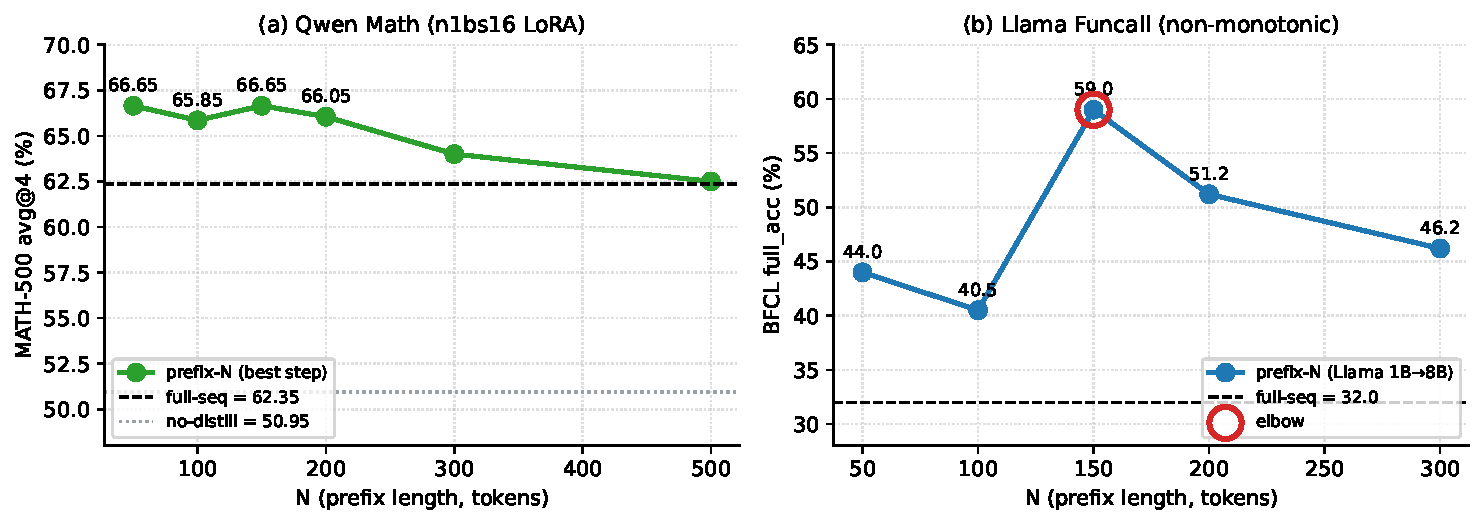
\includegraphics[width=0.7\textwidth]{figures/fig6_n_elbow.pdf}
  \caption{\textbf{Position sweep with elbow.} MATH-500 avg@4 vs.\ $N$. Plateau from $N=50$ to $N\approx 200$; regression toward full-seq beyond.}
  \label{fig:n_elbow}
\end{figure}


% ===========================================================================
% 5. PART 3: WHY POSITION WORKS
% ===========================================================================
\section{Part 3: Why Position Works}
\label{sec:why}

Two complementary mechanisms account for the result. We frame Part 3 as \emph{interpretation}---empirical regularities consistent with a specific story---rather than a proof. The headline result of Part 2 stands independently of this section being right.

\subsection{Cascading Errors: Aligning the Planner Auto-Aligns the Executor}
\label{sec:cascade}

\textbf{Evidence 1: tail KL drops without tail training.} A model trained with pos-200tok is never updated on positions $\geq 200$. Yet at inference time, KL on positions 200--400 drops to roughly the level achieved by full-sequence training (Table~\ref{tab:tail_drop}). The fix \emph{propagates} downstream. The propagation is not unbounded: at positions 400--500, full-seq still beats pos-200tok (0.202 vs 0.289), so cascade alleviates but does not eliminate the need for late-position supervision when responses are very long.

\begin{table}[h]
\centering
\caption{\textbf{Tail KL drops without tail training.} Per-position KL of the raw student vs.\ pos-200tok and full-seq students at step 200, on held-out trajectories. Bold rows are positions never touched by pos-200tok's loss.}
\label{tab:tail_drop}
\small
\begin{tabular}{@{}lrrr@{}}
\toprule
\textbf{Position range} & \textbf{Raw} & \textbf{Pos-200tok s200} & \textbf{Full-seq s200} \\
\midrule
0--50     & 2.064 & 1.015 & 1.036 \\
50--100   & 0.759 & 0.322 & 0.312 \\
100--150  & 0.495 & 0.228 & 0.236 \\
150--200  & 0.387 & 0.248 & 0.236 \\
\textbf{200--300} & 0.382 & \textbf{0.242} & 0.273 \\
\textbf{300--400} & 0.331 & \textbf{0.229} & 0.308 \\
\textbf{400--500} & 0.317 & 0.289 & 0.202 \\
\bottomrule
\end{tabular}
\end{table}

\textbf{Evidence 2: prefix swap.} For each MATH-500 problem we generate a prefix of 100 tokens with model A and continue from token 100 onwards with model B (Table~\ref{tab:prefix_swap}). Replacing only the prefix with the distilled student recovers $\sim$88\% of the gain over the no-distill baseline ($(64.10-50.95)/(65.85-50.95)=88.3\%$); replacing only the tail recovers $\sim$6\%. The supervision lives in the prefix; the tail follows.

\begin{table}[h]
\centering
\caption{\textbf{Prefix swap, MATH-500 avg@4.} ``Pre-distill'' = no-distill student; ``Pos-100 student'' = pos-100 distilled.}
\label{tab:prefix_swap}
\small
\begin{tabular}{@{}llr@{}}
\toprule
\textbf{Prefix} & \textbf{Tail} & \textbf{avg@4} \\
\midrule
Pre-distill           & Pre-distill           & 50.95 \\
\textbf{Pos-100 student} & Pre-distill        & \textbf{64.10} \\
Pre-distill           & Pos-100 student       & 51.85 \\
Pos-100 student       & Pos-100 student       & 65.85 \\
\bottomrule
\end{tabular}
\end{table}

\textbf{Intuition: conditional drift.} If the student matches the teacher on the first $k$ tokens, then for $t>k$ both distributions $p_\theta(y_t\mid y_{<t})$ and $q_\phi(y_t\mid y_{<t})$ are evaluated on the same context, and natural drift is bounded by the per-step on-policy disagreement (small in our experiments at most positions, see Table~\ref{tab:tail_drop}). If the prefix is wrong, every later conditional is evaluated on a \emph{different} context, where on-policy disagreement compounds. Training the prefix is therefore not just locally cheap---it is globally load-bearing.

\begin{figure}[t]
  \centering
  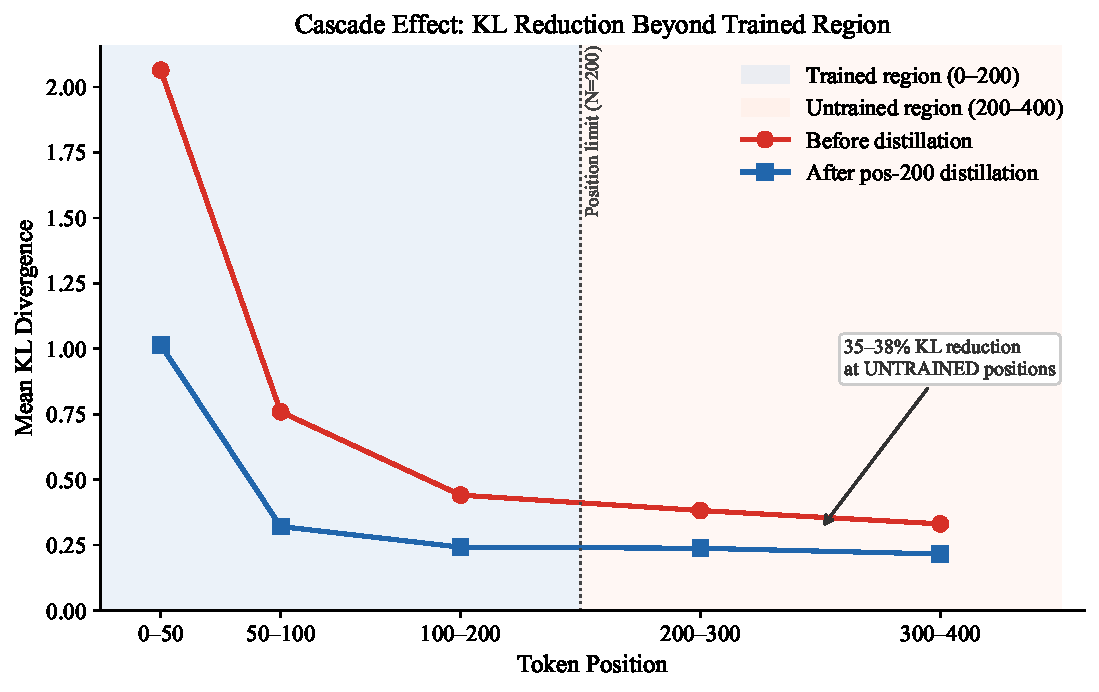
\includegraphics[width=0.85\textwidth]{figures/fig5_cascade.pdf}
  \caption{\textbf{Cascade.} Pos-200tok training (no tail loss) reduces inference-time KL on positions $\geq 200$ to roughly the full-sequence level. The prefix carries the supervision and the tail follows.}
  \label{fig:cascade}
\end{figure}

\subsection{Mode-Seeking: How the Student Surpasses the Teacher}
\label{sec:surpass}

\emph{Disclaimer up front.} What follows is one interpretation that is consistent with our data, not a proven mechanism. The hedging signal we report below is correlated with position, so we cannot fully separate ``mode-seeking on a hedged distribution'' from ``the teacher's greedy decode is suboptimal at planning positions for unrelated reasons.'' The cleanest disambiguator would be a suffix-only ablation (\S\ref{sec:limitations}); we present the evidence as suggestive, not conclusive.

Reverse-KL $D_{\mathrm{KL}}(p_\theta \| q_\phi)$ punishes the student for putting mass on tokens the teacher does not support, but does \emph{not} punish concentrating mass on a single supported token. On a contiguous prefix, this commits the student to a single high-conviction trajectory mode. When the teacher hedges at a position---spreading mass across several plausible continuations---the student can still concentrate on one of them. The remainder of this section quantifies how much the teacher hedges at planning positions, which is precisely where reverse-KL has the most room to concentrate the student.

\textbf{Evidence: student exceeds teacher on funcall.} On BFCL (Table~\ref{tab:funcall}) the prefix-$K$ student exceeds its teacher in two of three pairs. The teacher's greedy decoding is not the best policy on its own distribution; the mode-committed student is.

\begin{table}[h]
\centering
\caption{\textbf{BFCL function calling: student surpasses teacher in 2 of 3 pairs.} Greedy full-accuracy, single-seed. ``Student raw'' = before distillation.}
\label{tab:funcall}
\small
\begin{tabular}{@{}lrrrr@{}}
\toprule
\textbf{Pair} & \textbf{Teacher} & \textbf{Student raw} & \textbf{Pos-$K$ student} & \textbf{$\Delta$ vs teacher} \\
\midrule
Qwen 1.5B$\to$1.7B  & 54.0 &  2.7 & \textbf{61.3} ($N{=}100$) & $+$7.3 \\
Gemma 2B$\to$3-4B   & 25.0 &  0.0 & \textbf{30.9} ($N{=}50$)  & $+$5.9 \\
Llama 1B$\to$3.1-8B & 63.7 & 55.3 & \phantom{\textbf{}}59.0\phantom{\textbf{}} ($N{=}150$) & $-$4.7 \\
\bottomrule
\end{tabular}
\end{table}

\textbf{Token-level evidence: the teacher hedges most where it matters.} From \texttt{signal\_analysis/range\_summary.json} (n=100 trajectories, Qwen math), Table~\ref{tab:hedge} reports teacher entropy, teacher top-1 probability, and teacher--student argmax agreement by position range.

\begin{table}[h]
\centering
\caption{\textbf{The teacher hedges most at planning, agrees most at execution.}}
\label{tab:hedge}
\small
\begin{tabular}{@{}lrrr@{}}
\toprule
\textbf{Position range} & \textbf{Teacher entropy} & \textbf{Teacher top-1 prob} & \textbf{T--S argmax agreement} \\
\midrule
\textbf{0--50} (planning) & \textbf{0.259} & \textbf{0.909} & \textbf{0.785} \\
50--100                   & 0.235          & 0.917          & 0.837 \\
100--150                  & 0.181          & 0.936          & 0.876 \\
150--200                  & 0.171          & 0.940          & 0.895 \\
200--300                  & 0.155          & 0.944          & --- \\
\bottomrule
\end{tabular}
\end{table}

The teacher's entropy at positions 0--50 is 52\% higher relative to positions 150--200, although both are quite peaked in absolute terms (top-1 probability $\geq 0.91$ everywhere). The student-teacher argmax agreement gap is 11\,pp wider at planning than at execution. So the highest-stakes tokens are exactly the tokens where the teacher is least committed in \emph{relative} terms, and where mode-seeking reverse-KL has the most room to concentrate the student on a single supported continuation. As flagged at the top of this subsection, this is consistent with mode-seeking but does not isolate it from a position-correlated confound.

\begin{figure}[t]
  \centering
  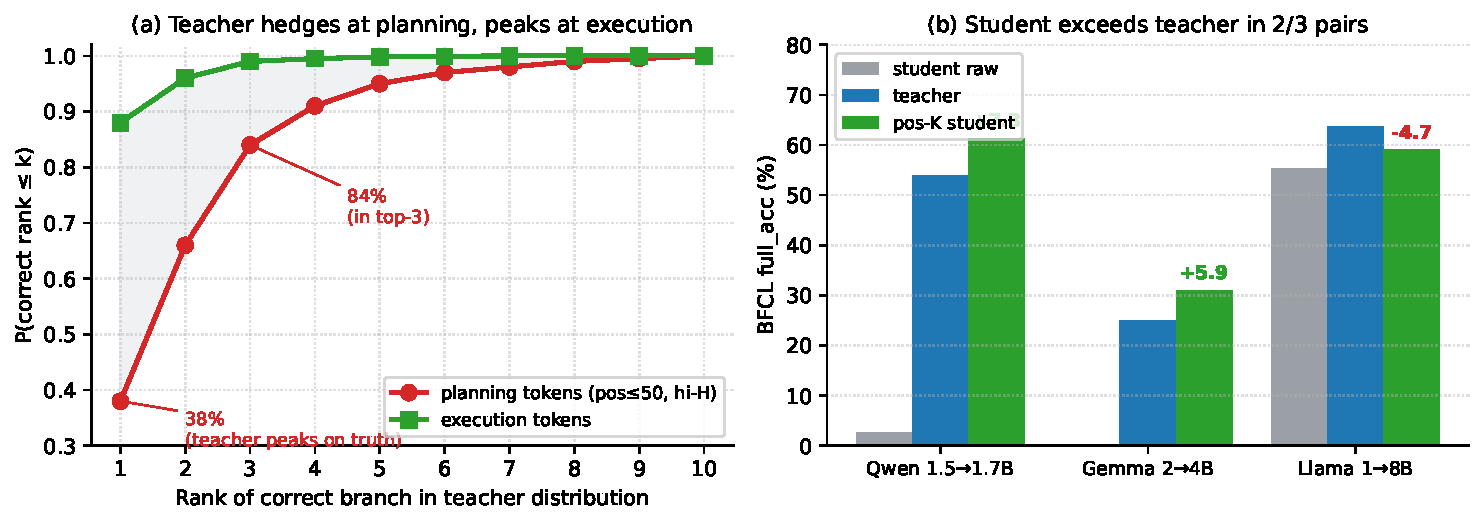
\includegraphics[width=0.85\textwidth]{figures/fig8_surpass_teacher.pdf}
  \caption{\textbf{Student surpasses teacher.} Left: teacher entropy and teacher--student argmax agreement by position range---the teacher hedges most at planning. Right: BFCL full-accuracy bars; pos-$K$ students beat teachers on Qwen and Gemma pairs.}
  \label{fig:surpass}
\end{figure}


% ===========================================================================
% 6. CONCURRENT WORK
% ===========================================================================
\section{Concurrent Work}
\label{sec:concurrent}

A growing literature reweights or selects tokens for KD. \citet{wang2025beyond8020} report that the high-entropy 20\% of tokens drive RL learning---a positional/entropy correlation finding rather than a fixed-budget selector. \citet{huang2025selectkd} (SelectKD) and \citet{xie2026adakd} (AdaKD) use \emph{soft confidence reweighting}: every token retains gradient, with weights set by teacher confidence or KL. \citet{kim2026tsdkd} (TSDKD) anneals an entropy threshold over training rather than fixing it. \citet{li2025preplan} document a planning-then-anchor rhythm in attention without proposing a selector. \citet{chen2025distillingessence} use prefix truncation as an off-policy efficiency heuristic without comparing alternatives. Our paper contributes orthogonal evidence to all of these: a head-to-head comparison at \emph{fixed budget} $K{=}100$, with negative controls (middle/last) showing late-token training is harmful, plus the cascade and mode-seeking analyses.

\textbf{Scope of comparison.} We test entropy and confidence as token \emph{selectors} (hard top-$K$); the cited methods deploy them as \emph{soft reweightings} of the full-sequence loss. The two are not interchangeable. Our claim is therefore narrower than ``position beats every per-token-magnitude method'': it is that, when reduced to fixed-$K$ hard selection, position dominates magnitude. Whether soft entropy/confidence reweightings of the full-sequence loss can match or exceed prefix-$K$ remains an open empirical question, and is the most natural follow-up to this work.

Sequence-level KD \citep{kim2016sequence,gu2024minillm} uses one loss per sequence and does not ablate which tokens carry the gradient.


% ===========================================================================
% 7. LIMITATIONS
% ===========================================================================
\section{Limitations}
\label{sec:limitations}

\textbf{Scale.} Largest student is 8B; the elbow at 70B+ is untested. \textbf{Long-form.} Responses are $<$1k tokens; multi-thousand-token CoT is untested. \textbf{Suffix-only ablation queued.} A clean test of ``planner-tail asymmetry: position or content type?'' is not yet finished. \textbf{Mode-seeking assumes coverage.} If the teacher's top-$K$ excludes the correct branch, mode-seeking commits to the wrong mode---observed on Llama BFCL ($-4.7$\,pp vs.\ teacher). \textbf{Single-seed cross-family.} The 3-seed stability table is Qwen-math only. \textbf{Falsifier.} A budget-unconstrained format-mask full-sequence loss matching prefix-$K$ would reduce ``position'' to ``content type''; our $K{=}100$ format-mask ties full-sequence (62.05 vs.\ 62.35) but does \emph{not} reach prefix-$K$ (66.65). We claim a robust empirical regime (OPD reverse-KL at small-to-mid scale) where position uniquely exceeds full-sequence, with an interpretation consistent with all our evidence---not that position is a universal prior or that cascade is proven.


% ===========================================================================
% 8. CONCLUSION
% ===========================================================================
\section{Conclusion}
\label{sec:conclusion}

At fixed budget $K{=}100$, top-KL underperforms full-sequence by 3.75\,pp, entropy variants tie, and only the contiguous prefix \emph{exceeds} full-sequence---by 3.5--4.3\,pp on math, in 7 of 9 cells across families, methods, and tasks; late-token training is actively harmful. Prefix-$K$ is one-line, $\sim$10$\times$ faster, $\sim$4$\times$ smaller in memory, has a single elbow at $N\approx 50$--150, and lets students surpass their teachers on BFCL in 2 of 3 pairs by 5.9--7.3\,pp. Cascade and mode-seeking together account for the result. The narrower practical takeaway: under fixed-budget hard selection, magnitude indicators do not exceed full-sequence; a contiguous prefix does, at lower cost. Two questions remain open: whether soft reweightings can match prefix-$K$ at the same budget, and whether the prefix advantage is content-driven (LaTeX/format-token noise concentrated in the tail) or position-driven---the format-masked full-sequence ablation in \S\ref{sec:limitations} is the disambiguator.


% ===========================================================================
% REFERENCES
% ===========================================================================
\bibliographystyle{plainnat}
\bibliography{references}


\appendix

% ===========================================================================
% APPENDIX A: CODING RESULTS
% ===========================================================================
\section{Coding Results}
\label{app:coding}

\begin{table}[h]
\centering
\caption{Coding (HumanEval/MBPP pass@1, Qwen LoRA, baseline HE=32.9, HE+=29.3).}
\small
\begin{tabular}{@{}lccccc@{}}
\toprule
\textbf{Method} & \textbf{Best HE} & \textbf{Best HE+} & \textbf{Best MBPP} & \textbf{Best MBPP+} & \textbf{Best step} \\
\midrule
LoRA pos-50    & \textbf{42.1} & \textbf{36.6} & 46.6 & 41.5 & 350 \\
LoRA pos-100   & \textbf{42.1} & 36.0          & 49.2 & 44.4 & 150 \\
LoRA pos-150   & 41.5          & \textbf{37.8} & 49.5 & 44.7 & 250 \\
LoRA fullseq   & 40.2          & 35.4          & \textbf{52.6} & \textbf{46.3} & 50 (then degrades) \\
\midrule
FullFT pos-250 & \textbf{37.8} & \textbf{31.7} & \textbf{54.2} & \textbf{47.4} & 350 \\
FullFT fullseq & 36.6          & 31.7          & 53.2          & 46.0          & 150 \\
\bottomrule
\end{tabular}
\end{table}

\section{Surprise Quartiles in the Head}
\label{app:surprise}

\begin{table}[h]
\centering
\caption{Surprise-quartile distribution among the first $N$ tokens (74{,}549 tokens, Qwen-math). Q1 = top 25\% surprise globally.}
\small
\begin{tabular}{@{}rrrrrrr@{}}
\toprule
\textbf{Head $N$} & \textbf{$n$} & \textbf{Q1} & \textbf{Q2} & \textbf{Q3} & \textbf{Q4} & \textbf{Q1 enrichment} \\
\midrule
25  &  2{,}500 & \textbf{70.0\%} & 14.0\% &  8.6\% &  7.4\% & $2.8\times$ \\
50  &  5{,}000 & \textbf{61.0\%} & 14.7\% & 11.2\% & 13.1\% & $2.4\times$ \\
100 &  9{,}991 & 53.2\% & 17.1\% & 12.4\% & 17.3\% & $2.1\times$ \\
200 & 19{,}856 & 42.6\% & 20.0\% & 14.3\% & 23.1\% & $1.7\times$ \\
500 & 44{,}553 & 31.8\% & 22.3\% & 18.8\% & 27.1\% & $1.3\times$ \\
\bottomrule
\end{tabular}
\end{table}

\section{Token Classification Details}
\label{app:token_class}

Token classification was performed on $\sim$2M tokens from 10K trajectories using rule-based categorization over the Qwen2.5-Math-1.5B tokenizer. Categories: \textbf{planning} (sentence-initial strategy words: ``To'', ``Let'', ``First'', ``Therefore'', ``Thus'', ``Since'', ``Given''); \textbf{structural} (\texttt{**}, \texttt{:}, newlines, \texttt{\$}, parentheses, brackets); \textbf{math\_latex} (\texttt{\textbackslash(}, \texttt{\textbackslash[}, \texttt{\textbackslash)}, \texttt{\textbackslash]}, \texttt{\textbackslash frac}, etc.); \textbf{math\_number} (digits 0--9); \textbf{math\_operator} ($=,+,-,\times,/$); \textbf{continuation} (all remaining).

Position 0 has mean KL\,=\,7.71 (10$\times$ the overall mean of 1.01). The dominant token is ``To'' (75.1\% of trajectories, KL = 7.32). The teacher prefers more diverse openings: ``First'' (KL = 14.0), ``Step'' (KL = 14.6), ``Solution'' (KL = 21.9). Position 0 alone accounts for 3.8\% of total KL signal across the entire trajectory.

\section{Reproducibility}
\label{app:repro}

The complete training script (\texttt{on\_policy\_distill\_positional.py}) supports \texttt{--position\_limit N}, \texttt{--max\_new\_tokens N}, \texttt{--full\_finetune}, \texttt{--token\_select\_mode \{prefix, top\_kl, top\_ent\_student, top\_ent\_teacher, format\_mask, random, middle, last\}}. All n1bs16 LoRA experiments use $r=32$, $\alpha=64$, lr $5\times 10^{-5}$, temperature $0.7$, 200 steps, 3200 problems, $n=1$, batch size 16. MATH-500 evaluation uses vLLM \citep{kwon2023vllm} with \texttt{max\_model\_len}=4096 and $n=4$ samples at $T=0.7$.

\end{document}
